\chapter{Watched Cricket match}
India and Australia match is always wonderful to watch. While Australia was 170/10
in 17.4 over, India scored 172/4 in 15.5 over and won by 6 wickets.

Below is the line graph.

\begin{figure}[H]
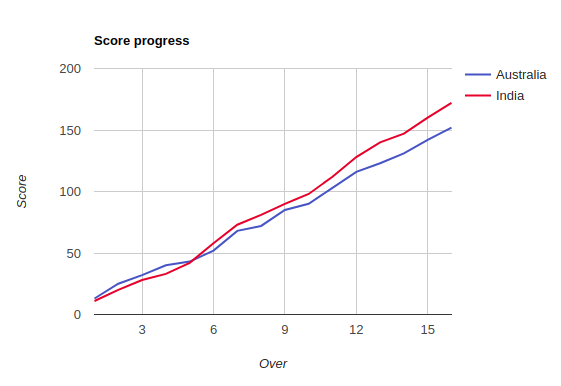
\includegraphics[scale=0.5]{line_graph.png}
\caption{Line graph of India Vs Australia}
\end{figure}

Also the bar graph was like shown in figure 2.2 :-

\pgfplotstableread[row sep=\\,col sep=&]{
    over & aus 	& india	\\
    1    & 	13 	&	11 	\\
    2    & 	12  & 	9 	\\
    3    & 	7 	& 	8 	\\
    4    & 	8 	& 	5 	\\
    5    & 	3  	& 	9 	\\
    6    & 	9  	& 	16 	\\
    7	 &	16	&	15	\\
    8	 &	4	&	8	\\
    9	 &	13	&	9	\\
    10	 &	5	&	8	\\
    11	 &	13	&	14	\\
    12	 &	13	&	16	\\
    13	 &	7	&	12	\\
    14	 &	8	&	7	\\
    15	 &	11	&	13	\\
    16	 & 	10	&	12	\\
    17	 &	7	&	0	\\
    18	 &	11 	&	0	\\
    }\mydata

\begin{figure}
\begin{tikzpicture}
    \begin{axis}[
            ybar,          
            bar width=.2cm,
            width=\textwidth,
            height=.5\textwidth,
            legend style={at={(0.5,1)},
                anchor=north,legend columns=-1},  
            symbolic x coords={1,2,3,4,5,6,7,8,9,10,11,12,13,14,15,16,17,18},
        ]
        \addplot table[x=over,y=aus]{\mydata};
        \addplot table[x=over,y=india]{\mydata};
        \legend{Australia,India}
    \end{axis}
\end{tikzpicture}
\caption{Bar graph of India Vs Australia}
\end{figure}